\section{Simulation study}

The simulation uses a finite population of size \(N=20\) and a fixed sample size \(n=4\). In this diagnostic experiment two variables are generated. The ABC objective is the Horvitz--Thompson variance of the variable denoted by \(z\) in the notebook. The second variable, denoted by \(y\), is not optimized directly; it is used to check whether improving the design for \(z\) also improves, or damages, the variance for a related variable.

Three \(z\)-cases are considered. They are constructed so that the raw correlations with \(y\) are approximately
\[
    r(y,z)\in\{0,0.80,0.90\}.
\]
For each \(z\)-case, ten inclusion-probability scenarios are considered: the equal-probability design and nine unequal-probability designs labelled \(\pi_{0.10},\ldots,\pi_{0.90}\). The equal-probability case has \(\pi_k=n/N\). For every scenario, the population is ordered so that Vincent's monotonicity condition holds for the optimized variable:
\[
    \pi_1\geq\cdots\geq\pi_N,
    \qquad
    z_1/\pi_1<\cdots<z_N/\pi_N.
\]
The CaDSD Vincent start with \(\omega=0\) and \(\rho=0.5\) was checked against the real-valued \(\Ppi\) reference. For the optimized variable, the reported efficiency is
\[
    \frac{V_{\Ppi_z}(z)}{V_K(z)}.
\]
For the companion variable \(y\), the denominator is its own Vincent reference based on the \(y/\pi\) ordering, so the corresponding diagnostic efficiency is
\[
    \frac{V_{\Ppi_y}(y)}{V_K(y)}.
\]
A value larger than one means that the candidate kernel has smaller computed HT variance than the relevant real-valued \(\Ppi\) reference.

The ABC run uses the following settings:
\[
\begin{gathered}
N=20,\quad n=4,\quad
\text{maximum iterations}=1000,\quad
\text{threshold}=3.5,\\
\text{colony size}=10,\quad
\text{limit}=20.
\end{gathered}
\]
The search is stopped separately for each scenario. It stops as soon as the \(z\)-efficiency reaches or exceeds \(3.5\), or after \(1000\) iterations if the threshold is not reached. This stopping rule avoids running far beyond the first practically meaningful improvement and makes the results easier to compare across scenarios.

\begin{figure}[!htbp]
\centering
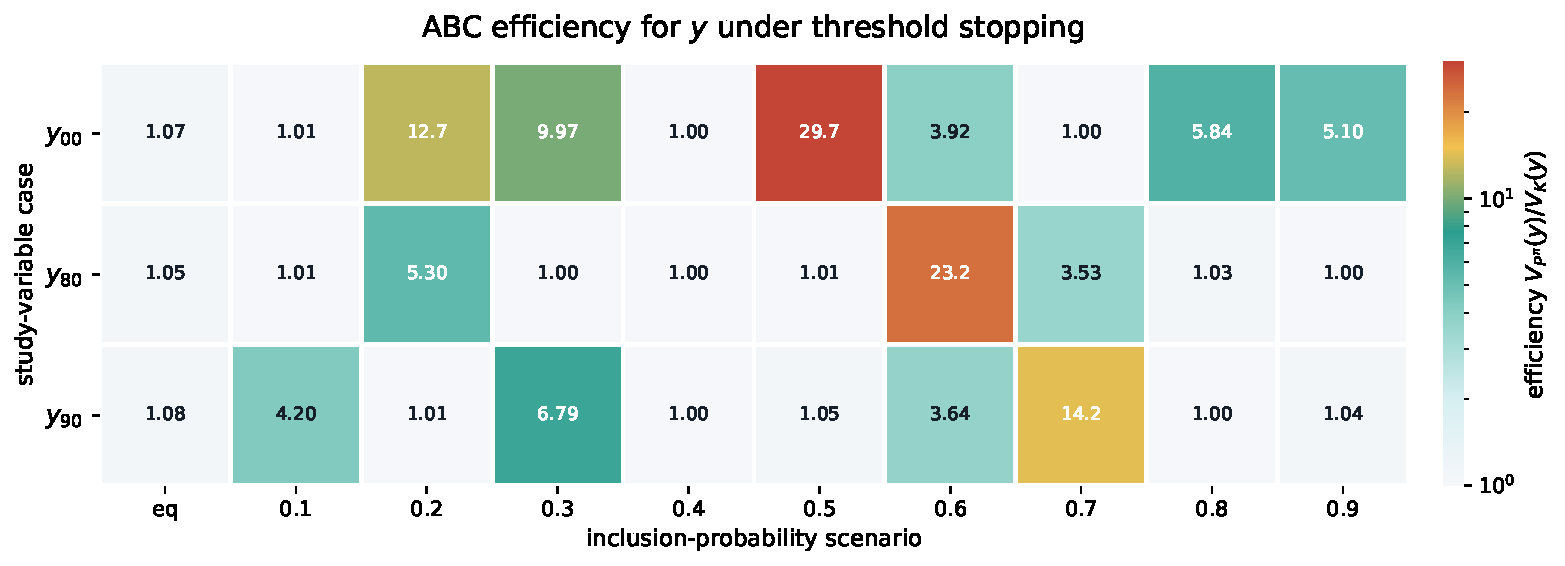
\includegraphics[width=0.95\textwidth]{abc_threshold_efficiency_heatmap_pretty.pdf}
\caption{Efficiency for the optimized variable \(z\) under threshold stopping. Each cell reports \(V_{\Ppi_z}(z)/V_K(z)\). Light cells close to one indicate that no meaningful improvement over the real-valued \(\Ppi\) reference was found. Colored cells indicate scenarios where ABC found a candidate complex kernel with smaller computed HT variance.}
\label{fig:abc-threshold-efficiency}
\end{figure}

\begin{figure}[!htbp]
\centering
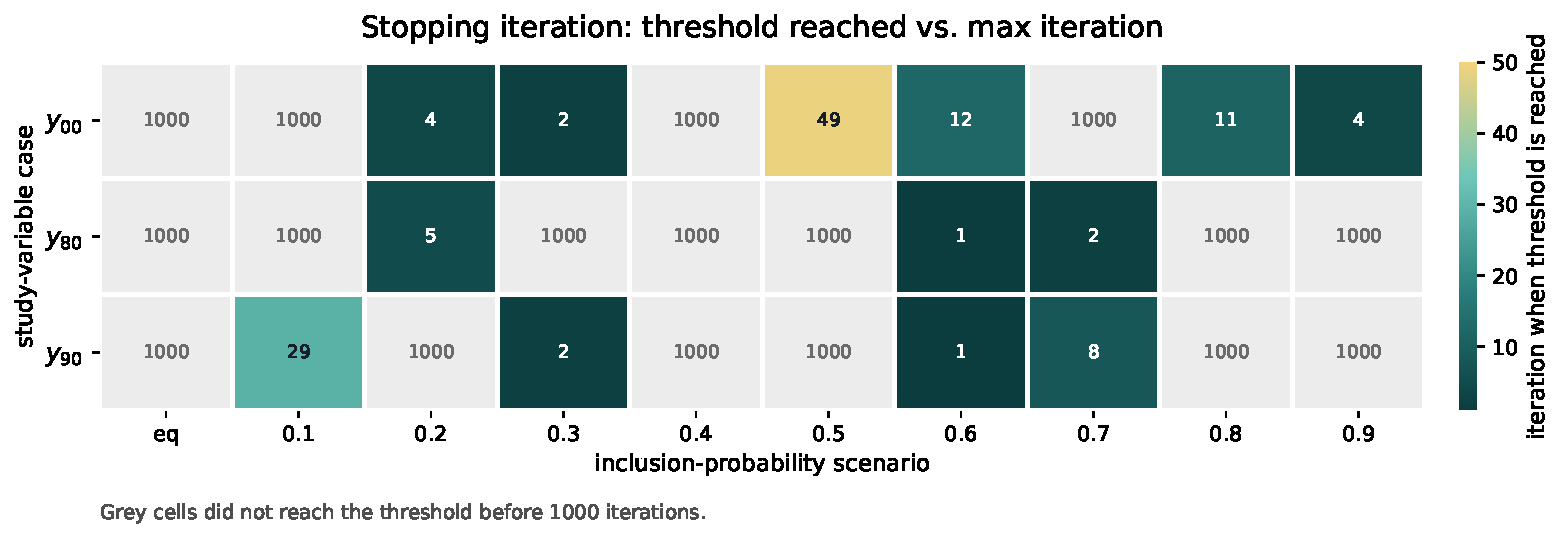
\includegraphics[width=0.95\textwidth]{abc_threshold_stop_iteration_heatmap_pretty.pdf}
\caption{Iteration at which the search stopped. Colored cells reached the \(z\)-efficiency threshold before \(1000\) iterations; the number is the first reported stopping iteration. Grey cells did not reach the threshold and therefore stopped at the maximum iteration limit.}
\label{fig:abc-threshold-stopping}
\end{figure}

Figures~\ref{fig:abc-threshold-efficiency} and~\ref{fig:abc-threshold-stopping} summarize the optimization results for \(z\). In 13 of the 30 scenarios, ABC reaches the threshold before the maximum iteration limit. Several of these improvements occur very quickly, sometimes within only a few iterations. In the remaining scenarios, the efficiency remains close to one even after \(1000\) iterations. This suggests two qualitatively different regimes: some combinations of \(z\) and \(\pi\) allow the complex CaDSD parametrization to improve rapidly on the real-valued reference, while others appear much more resistant to improvement.

\begin{figure}[!htbp]
\centering
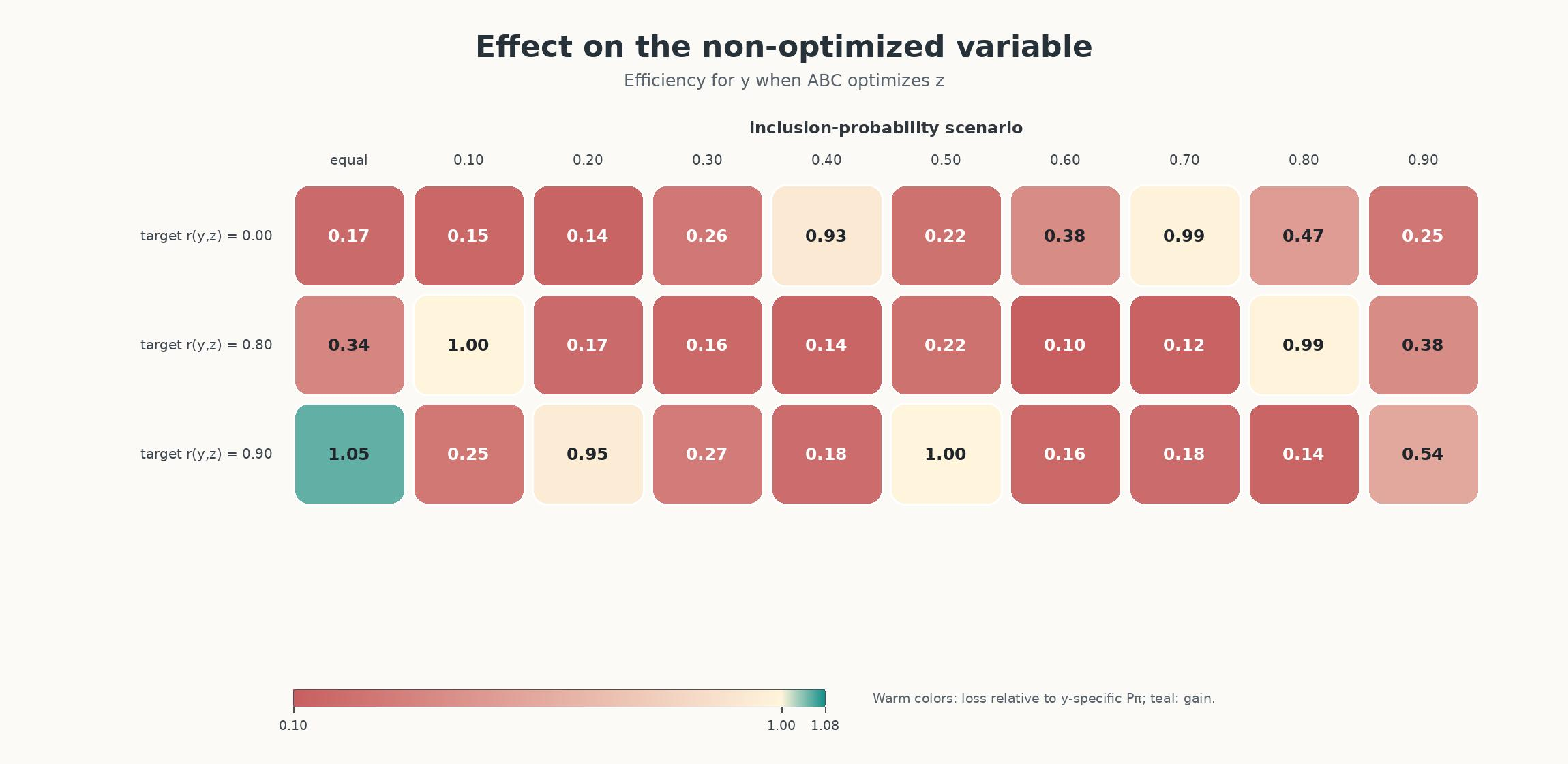
\includegraphics[width=0.95\textwidth]{abc_threshold_auxiliary_efficiency_heatmap_pretty.pdf}
\caption{Effect of the \(z\)-optimized kernel on the companion variable \(y\). Each cell reports \(V_{\Ppi_y}(y)/V_K(y)\), where \(\Ppi_y\) is the Vincent reference built from the \(y/\pi\) ordering. Values below one show that the \(z\)-optimized kernel is worse than the \(y\)-specific real-valued reference for estimating \(y\).}
\label{fig:abc-auxiliary-efficiency}
\end{figure}

\begin{figure}[!htbp]
\centering
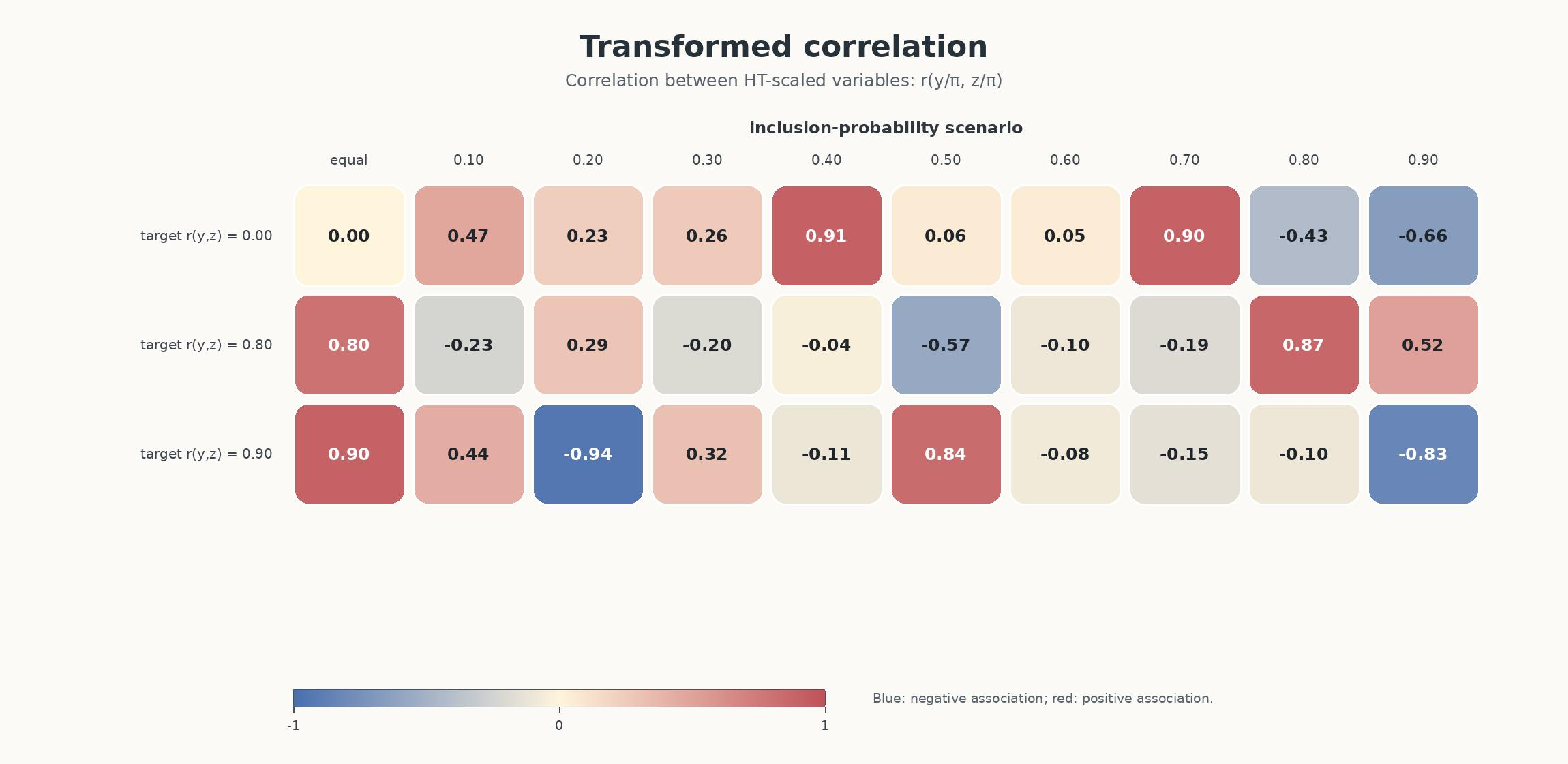
\includegraphics[width=0.95\textwidth]{abc_threshold_transformed_correlation_heatmap_pretty.pdf}
\caption{Correlation between the HT-scaled variables \(y/\pi\) and \(z/\pi\). The raw correlation \(r(y,z)\) is fixed by row, but the transformed correlation can change substantially once the inclusion probabilities are introduced.}
\label{fig:abc-transformed-correlation}
\end{figure}

Figures~\ref{fig:abc-auxiliary-efficiency} and~\ref{fig:abc-transformed-correlation} explain why improvement for \(z\) does not automatically transfer to \(y\). Even when the raw correlation \(r(y,z)\) is high, the transformed correlation \(r(y/\pi,z/\pi)\) can be weak or negative. Since the HT variance is driven by the scaled quantities, optimizing the design for \(z\) can leave the variance for \(y\) almost unchanged or make it worse relative to the \(y\)-specific Vincent reference. This is visible in Figure~\ref{fig:abc-auxiliary-efficiency}: most cells are below one, with only a few cases near or slightly above one.

The results should still be interpreted as numerical evidence rather than as a theoretical optimum. They show that, under the CaDSD parametrization and the numerical checks used in the notebook, ABC can find complex Hermitian kernels with the prescribed diagonal and smaller computed HT variance for the optimized variable \(z\) than the real-valued \(\Ppi\) reference. The auxiliary-variable heatmap shows that this gain is target-specific. The candidate kernels should be checked independently for admissibility, projection accuracy, and variance calculation before making a final claim.
